\documentclass[10pt,a4paper]{article}
\usepackage[utf8]{inputenc}
\usepackage[OT4]{fontenc}
\usepackage{amsmath}
\usepackage{amsfonts}
\usepackage{amssymb}
\usepackage{titling}
\usepackage{anysize}
\usepackage{parskip}
\usepackage{graphicx}
\usepackage[polish]{babel}
\usepackage{float}
% some settings'

\setlength{\droptitle}{-2cm}
\preauthor{}
\DeclareRobustCommand{\authorthing}{
\begin{center}
\begin{tabular}{cc}
\large{Dominik Galewski} & \large{Jakub Woźniak} \\
106575 & 109686\\
dominik.galewski@student.put.edu.pl & jakub.l.wozniak@student.put.edu.pl
\end{tabular}\\
\vspace{8pt}
\large{Prowadzący: mgr inż. Mateusz Cicheński}\\
Wydział Informatyki Politechniki Poznańskiej
\end{center}}
\author{\authorthing}
\date{18 listopada 2013}
\postauthor{}
\title{Trouble in Lecture Center\\\small{\MakeUppercase{Gra dungeon explorer}}\\\Large{Laboratorium Programowania Obiektowego}}
\marginsize{2cm}{2cm}{1cm}{1cm}

\setlength{\parindent}{0pt}
% document
\begin{document}
\maketitle


\section{Wprowadzenie}
\textbf{Trouble in Lecture Center} to gra typu \textit{dungeon explorer}, w której wcielamy się w postać studenta informatyki. Odwiedzając kolejne lokacje znajdujące się w mrocznych podziemiach jego uczelni, próbujemy zmierzyć się ze wszystkimi przeciwnościami: analizą matematyczną, programowaniem deklaratywnym, systemami operacyjnymi czy metodami probabilistycznymi. Nasze decyzje wpływają na los studenta i wynik starć z przeciwnikami.


\section{Struktura projektu}
\subsection{Instrukcja kompilacji}
Projekt został napisany w języku C++ (standard C++11) przy użyciu biblioteki \textit{SFML} (http://sfml-dev.org) w wersji 2.0. Do kompilacji wymagany jest kompilator g++ w wersji 4.8. Dostarczony plik \textit{Makefile} pozwala na skompilowanie projektu przy pomocy polecenia \textit{make}. Plik wynikowy znajduje się w katalogu \textit{bin}. 

\subsection{Podział klas}
Rysunek \ref{uml-game} przedstawia podział klas związanych z rozgrywką. Główną klasę stanowi \textit{Entity}, która reprezentuje wszystkie elementy w grze, które mogą być narysowane na mapie i w interfejsie. Klasa \textit{Item} to przedmioty, które znajduje gracz podczas rozgrywki. Może je podnieść, użyć, niektóre także założyć i wykorzystać w walce. Klasa \textit{Player} dotyczy postaci, którą kierujemy. Jej pochodne to profesje, jedną z nich wybieramy na samym początku gry. Klasa \textit{NPC} to wszyscy przeciwnicy, których gracz napotka podczas rozgrywki. 
\begin{figure}
    \centering
    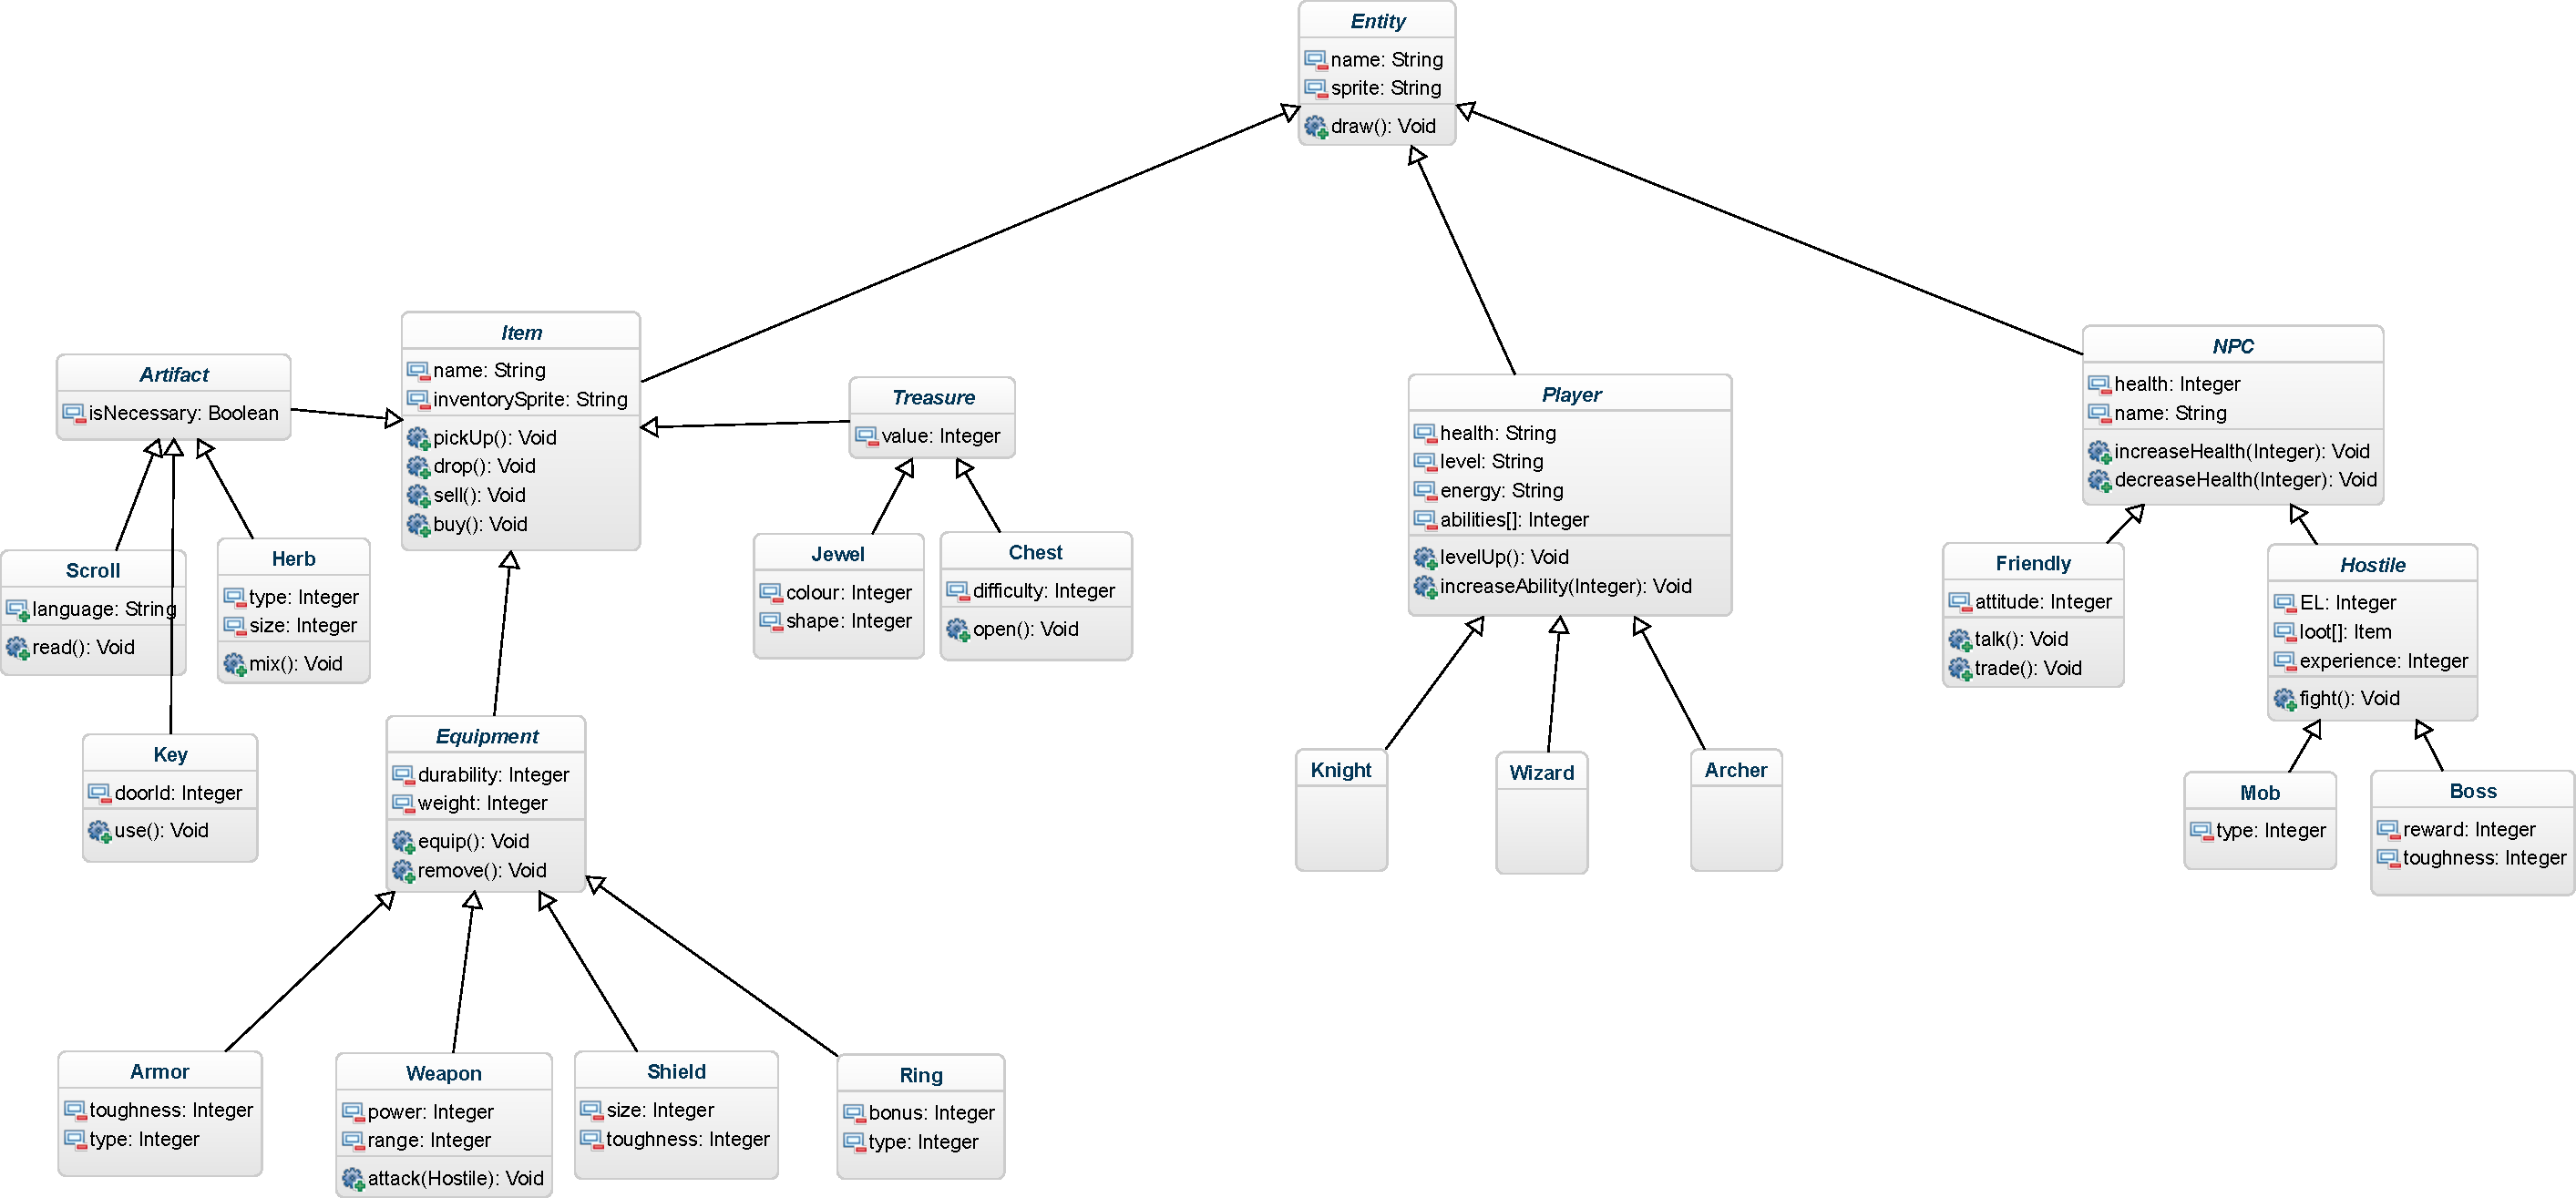
\includegraphics[width=\textwidth]{doc/uml/lc-ex-diag.pdf}
    \caption{diagram podziału klas związanych z rozgrywką}
    \label{uml-game}
\end{figure}

\section{Spis wymagań}
\subsection{Graficzny interfejs użytkownika}
Interfejs użytkownika został zrealizowany przy pomocy biblioteki \textit{SFML}. Wykorzystane elementy graficzne i dźwiękowe zostały wykonane przez nas lub są na wolnej licencji. Mapa zrealizowana jest w widoku ,,z lotu ptaka''.

\subsection{Wpływanie na rozgrywkę}
Użytkownik poruszając się po mapie, walcząc z przeciwnikami i zdobywając wyposażenie, udoskonala swoje umiejętności z różnych dziedzin, które pozwolą mu przejść do następnego etapu.

\subsection{Zapis stanu gry}
Użytkownik w każdym momencie gry ma możliwość zapisu aktualnego stanu celem późniejszego odtworzenia. Jest to zrealizowane przy pomocy osobnego menu uruchamianego poprzez naciśnięcie klawisza \textit{Esc}.

\end{document}
